\section{Week 1}
\textbf{\large Terminologies}
\begin{table}[h]
\begin{tabular}{|l|l|l|}
\hline
\textbf{Jargon} & \textbf{Symbol}    & \textbf{Unit} \\ \hline
Heat            & $Q$                & $[J]$         \\ \hline
Heat rate       & $\dot{Q}=Q/t$      & $[W]$         \\ \hline
Heat flux       & $q''=\dot{Q}/A$ & $[W/m^2]$      \\ \hline
\end{tabular}
\end{table}

\textbf{\large Mode of Heat Transfer}
\begin{itemize}
    \item \underline{\textbf{Conduction:}} Energy transfer from \color{red} more energetic \color{black} particles to \color{red} less energetic \color{black} particles of a substance; requires medium.
    
    \textbf{Fourier's law of heat conduction:}
    \begin{align*}
       \dot{Q} &= -kA\frac{T_2-T_1}{\Delta x} = -kA \frac{\Delta T}{\Delta x}, \; \; [W] \\
        q'' &= -k\frac{T_2-T_1}{\Delta x} = k \frac{T_1-T_2}{\Delta x}, \; \; [W/m^2]\\
        \text{where } k &= \text{thermal conductivity, [$W/m\cdot K$]}
    \end{align*}
    \begin{figure}[h]
        \centering
        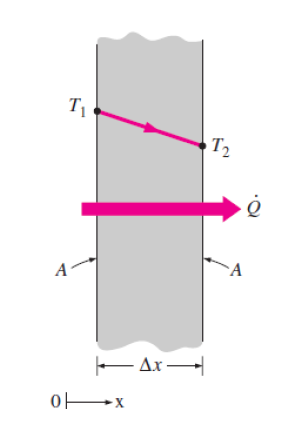
\includegraphics[width=0.5\linewidth]{images/conduction.png}
    \end{figure}
    \item \underline{\textbf{Convection:}} Energy transfer between a solid surface and an adjacent liquid/gas in motion; combined effects of \color{red} conduction \color{black} and \color{red} fluid motion \color{black}; requires medium.
    
    \textbf{Newton's Law of Cooling:}
    \begin{align*}
        \dot{Q} &= h A_s (T_s - T_{\infty}), \; \; [W] \\
        q'' &= h (T_s - T_{\infty}), \; \; [W/m^2] \\
        \text{where } T_s &= \text{temp. of the surface,} \\
        T_{\infty} &= \text{temp. of fluid far from surface,} \\
        A_s &= \text{surface area,} \\
        h &= \text{convection coefficient, [$W/m^2\cdot K$]}
    \end{align*}
    \item \underline{\textbf{Radiation:}} Energy that is emitted by matter and is transported as \color{red} electromagnetic waves / photons \color{black}; does not require medium.
    \begin{figure}[h]
        \centering
        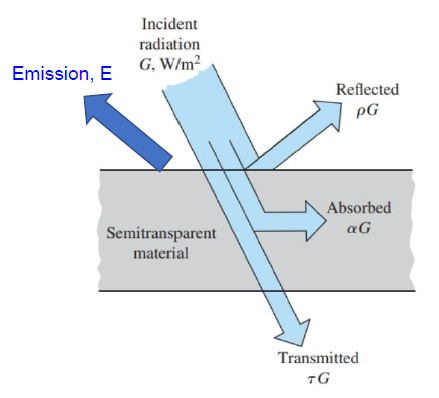
\includegraphics[width=0.75\linewidth]{images/radiation.png}
    \end{figure}
    \begin{align*}
        \rho + \alpha + \tau &= 1, \; \; \text{(for any medium)} \\
        \rho + \alpha &= 1, \; \; \text{(for opaque medium)} \\
        \text{where } \rho &= \text{fraction of G reflected,} \\
        \alpha &= \text{fraction of G absorbed,} \\
        \tau &= \text{fraction of G transmitted through the medium.}
    \end{align*}
    \textbf{Kirchoff's Law of Thermal Radiation:}
    \begin{equation*}
        \alpha = \epsilon \; \; \text{(for most cases)}
    \end{equation*}
    \textbf{Emissive Power E:} 
    \begin{align*}
        E &= \sigma \epsilon T_{s}^{4}, \; \; [W/m^2] \\
        \dot{Q}_E &= \sigma A_s \epsilon T_s^4, \; \; [W]\\
        \text{where } \sigma &= 5.67\times 10^{-8} \; W/m^2 K^4 \; \; \text{(Stefan-Boltzmann constant)} \\
        \epsilon &= \text{Emissivity} 
    \end{align*}
    \textbf{Irradiation G:}
    \begin{align*}
        G_{total} &= (\alpha + \beta + \tau) \sigma T_{surr}^4 \\
        &= \sigma T_{surr}^4 \\
        G_{absorbed} &= \alpha \sigma T_{surr}^4 \\
        &= \epsilon \sigma T_{surr}^4
    \end{align*}
    \textbf{Special case:} surface exposed to large surroundings of uniform temperature $T_{surr}$
    \begin{figure}[h]
        \centering
        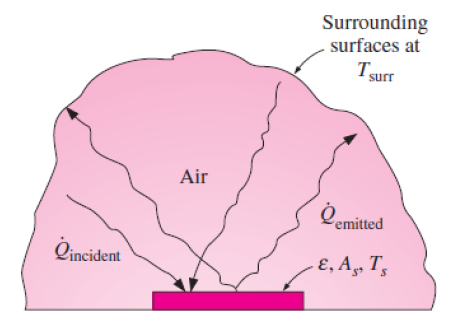
\includegraphics[width=0.7\linewidth]{images/radiation_special_case.png}
    \end{figure}
    \begin{align*}
        \dot{Q} &= E- G_{absorbed} \\
        &= A_s \left(\underbrace{\epsilon \sigma T_s^4}_{E} - \underbrace{\alpha \sigma T_{surr}^4}_{\alpha G}\right) \\
        &= \sigma A_s \epsilon (T_s^4 - T_{surr}^4)
    \end{align*}
    Alternatively,
    \begin{align*}
        \dot{Q} &= h_r A_s (T_s - T_{surr} ) \\
        \text{where } h_r &= \text{radiation heat transfer coefficient, W/$m^2$K}\\ 
        &=\epsilon \sigma (T_s + T_{surr})(T_s^2+T_{surr}^2)
    \end{align*}
    \item \textbf{\color{red}Overall\color{black}} heat flux for radiation:
    \begin{equation*}
        \dot{Q} = E + (\rho - \alpha - \tau) \cdot G
    \end{equation*}
    \item \textbf{\color{red}Net\color{black}} heat flux for radiation:
    \begin{align*}
        \dot{Q} &= \text{total leaving surface} - \text{total approaching surface} \\
        \dot{Q} &= E + (\rho+\tau ) G - G
    \end{align*}
\end{itemize}

\large\textbf{Heat Generation}
\begin{itemize}
    \item Unit of heat generation $\dot{g}$: [W/$m^3$]
    \item Rate of heat generation: $\dot{Q}=\dot{g}V$ [W]
    \item Surface Temperature: $T_s = T_{\infty}+\frac{\dot{g}V}{h A_s}$
    \item For \underline{\textbf{large plane wall}} of thickness $2L$:
    \begin{align*}
        A_s&=2A_{wall} \\
        V &=2LA_{wall} \\
        T_{\text{s,plane wall}} &= T_{\infty}+\frac{\dot{g}L}{h}
    \end{align*}
    \item For \underline{\textbf{solid cylinder}} of radius $r_o$:
    \begin{align*}
        A_s &= 2\pi r_o L \\
        V &=\pi r_o^2 L \\
        T_{\text{s,cylinder}} &= T_{\infty} + \frac{\dot{g}r_o}{2h}
    \end{align*}
    \item For \underline{\textbf{sphere}} of radius $r_o$:
    \begin{align*}
        A_s &= 4\pi r_o^2 \\
        V &= \frac{4}{3} \pi r_o^3 \\
        T_{\text{s,sphere}} &= T_{\infty} + \frac{\dot{g}r_o}{3h} 
    \end{align*}
\end{itemize}

\large\textbf{Max Temperature}
\begin{figure}[h]
    \centering
    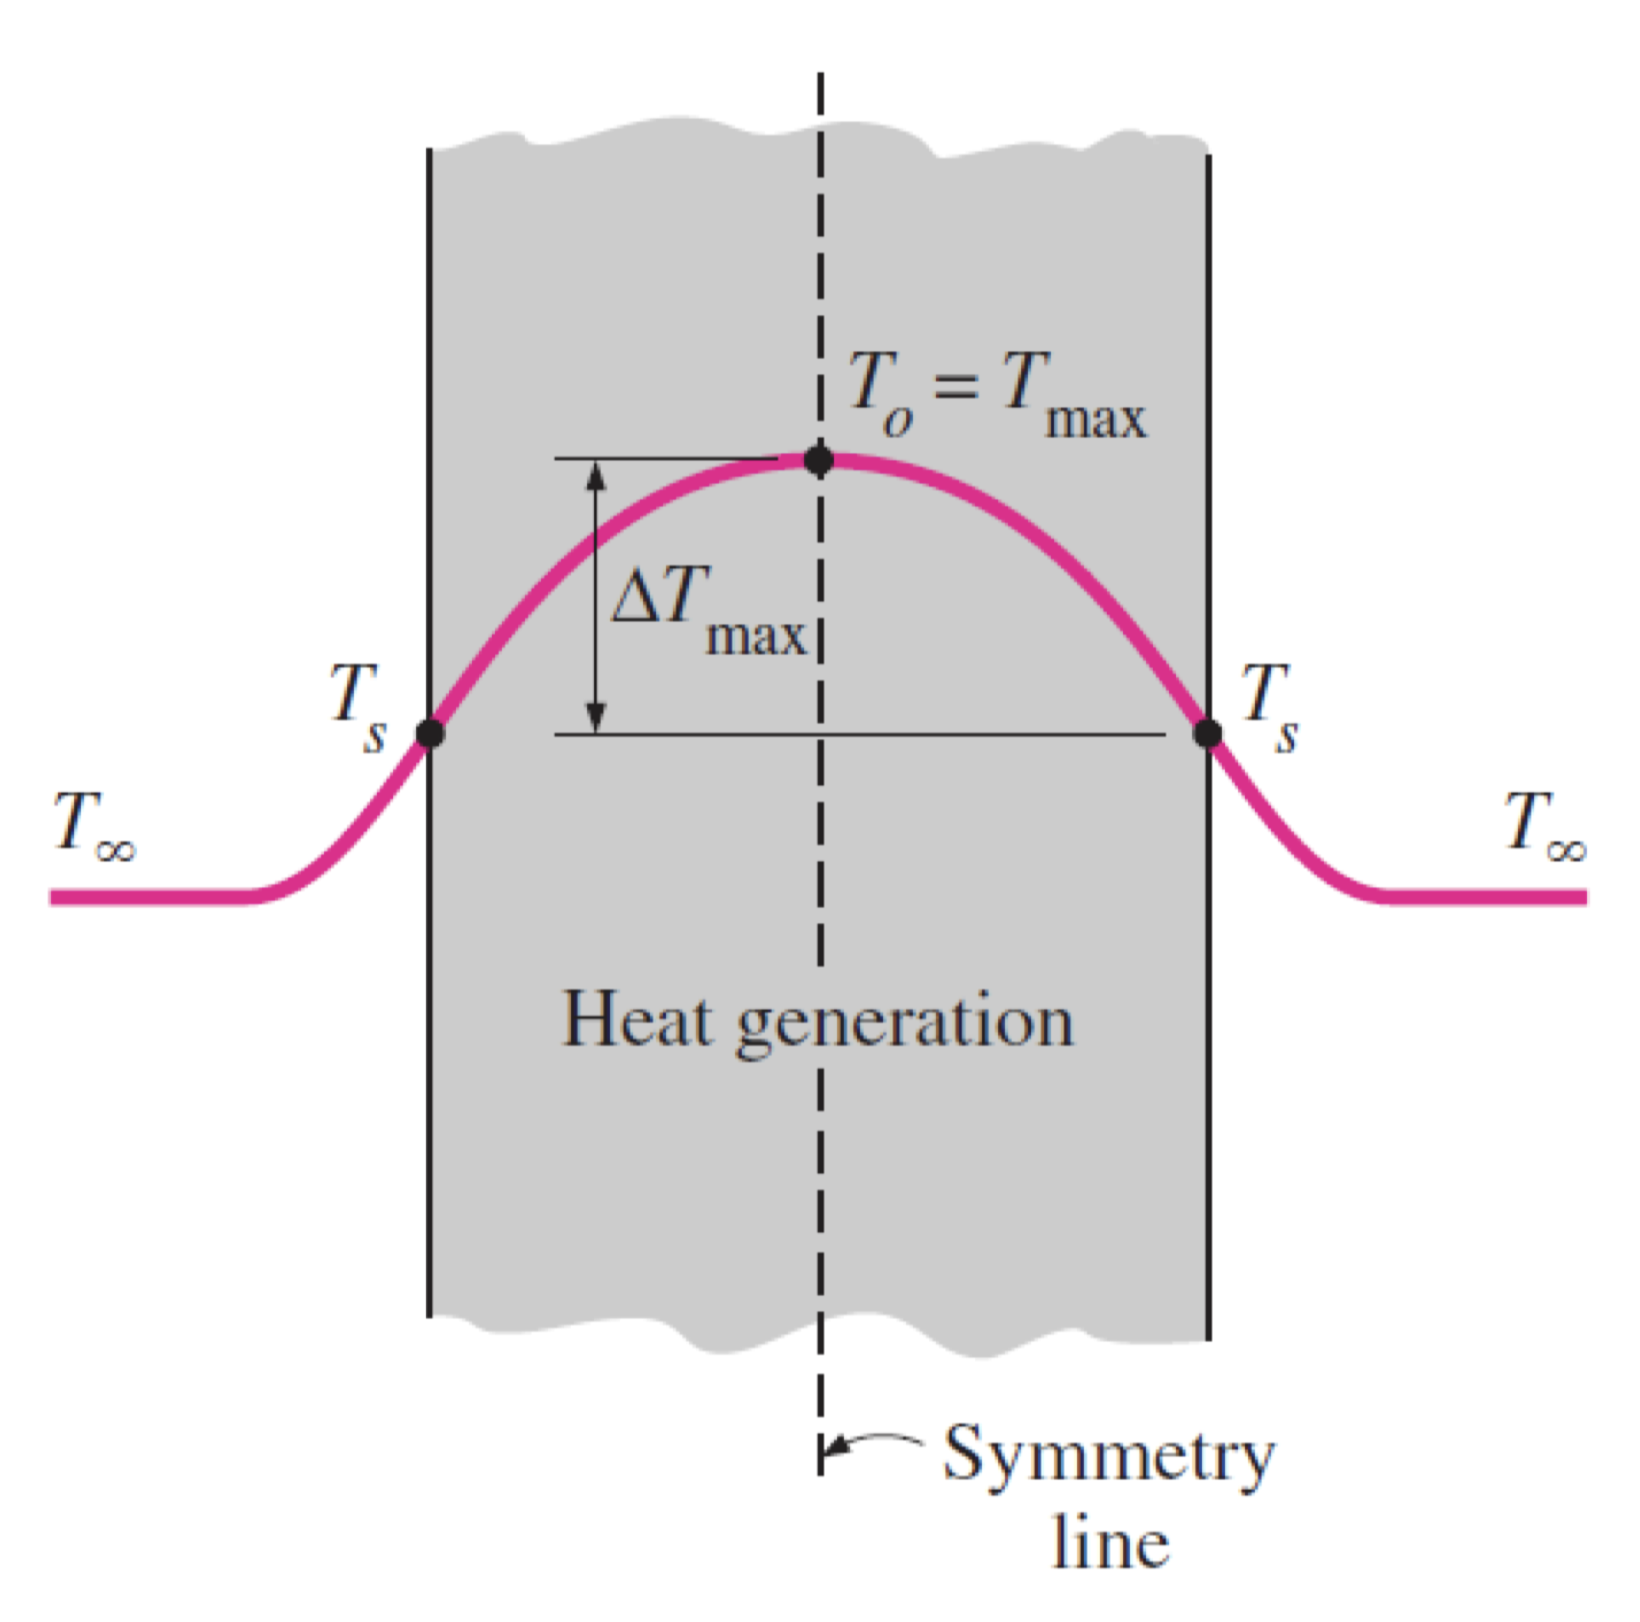
\includegraphics[width=0.75\linewidth]{images/heat_generation_max_temp.png}
\end{figure}

\begin{align*}
    \Delta T_{\text{max,cylinder}}&= T_o - T_s = \frac{\dot{g}r_o^2}{4k} \\
    \Delta T_{\text{max,plane wall}} &= \frac{\dot{g}L^2}{2k} \\
    \Delta T_{\text{max,sphere}} &= \frac{\dot{g}r_o^2}{6k}
\end{align*}

\large\textbf{Heat Equations}
\begin{enumerate}
    \item Heat conduction through \color{red} large plane wall: \color{black}
    \begin{equation*}
        \frac{\partial^2 T}{\partial x^2} + \frac{\dot{e}_g}{k} = \frac{1}{\alpha} \frac{\partial T}{\partial t}
    \end{equation*}
    \item Heat conduction in \color{red} long cylinder: \color{black}
    \begin{equation*}
        \frac{1}{r} \frac{\partial}{\partial r}\left(r \frac{\partial T}{\partial r}\right) + \frac{\dot{e}_g}{k} = \frac{1}{\alpha} \frac{\partial T}{\partial t}
    \end{equation*}
    \item Heat conduction in \color{red} sphere: \color{black}
    \begin{equation*}
        \frac{1}{r^2} \frac{\partial}{\partial r} \left( r^2 \frac{\partial T}{\partial r}\right) + \frac{\dot{e}_g}{k} = \frac{1}{\alpha} \frac{\partial T}{\partial t}
    \end{equation*}
\end{enumerate}

\large\textbf{Thermal Resistance}
\begin{itemize}
    \item Definition:
    \begin{align*}
        R &= \frac{\text{driving force}}{\text{transfer rate}} \\
        &= \frac{T_1 - T_2}{\dot{Q}}\;\; \text{ in [K/W]}
    \end{align*}
    \item Overall heat transfer coefficient UA$:=\frac{1}{\sum R_i}$
    \item For \color{red} plane walls: \color{black}
    \begin{align*}
        R_{cond} &= \frac{L}{kA_s} \\
        R_{conv} &= \frac{1}{h A_s} \\
        R_{rad} &= \frac{1}{h_r A_s}
    \end{align*}
    \item Example:
    \begin{itemize}
        \item In series:
        \begin{figure}[H]
            \centering
            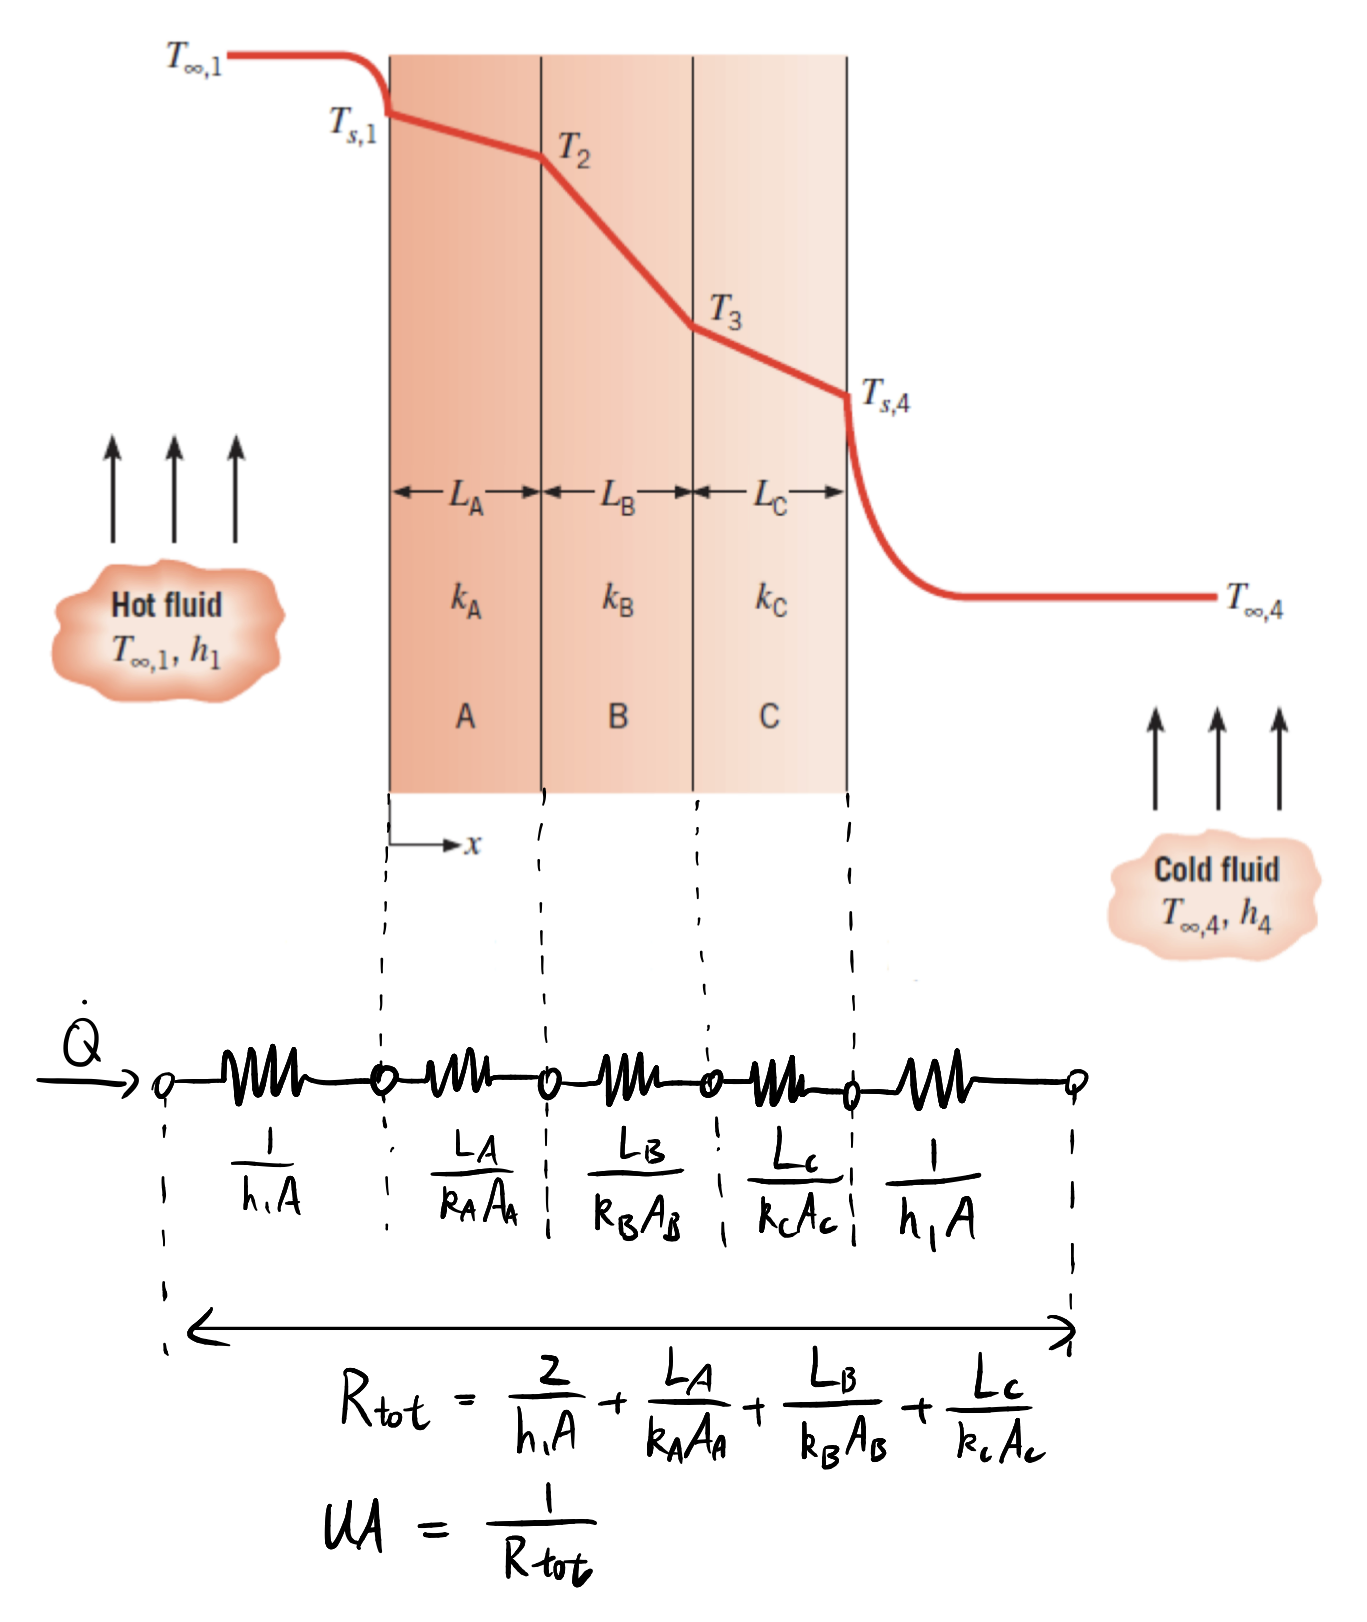
\includegraphics[width=0.85\linewidth]{images/thermal_resistance.png}
        \end{figure}
        \item In parallel:
        \begin{figure}[H]
            \centering
            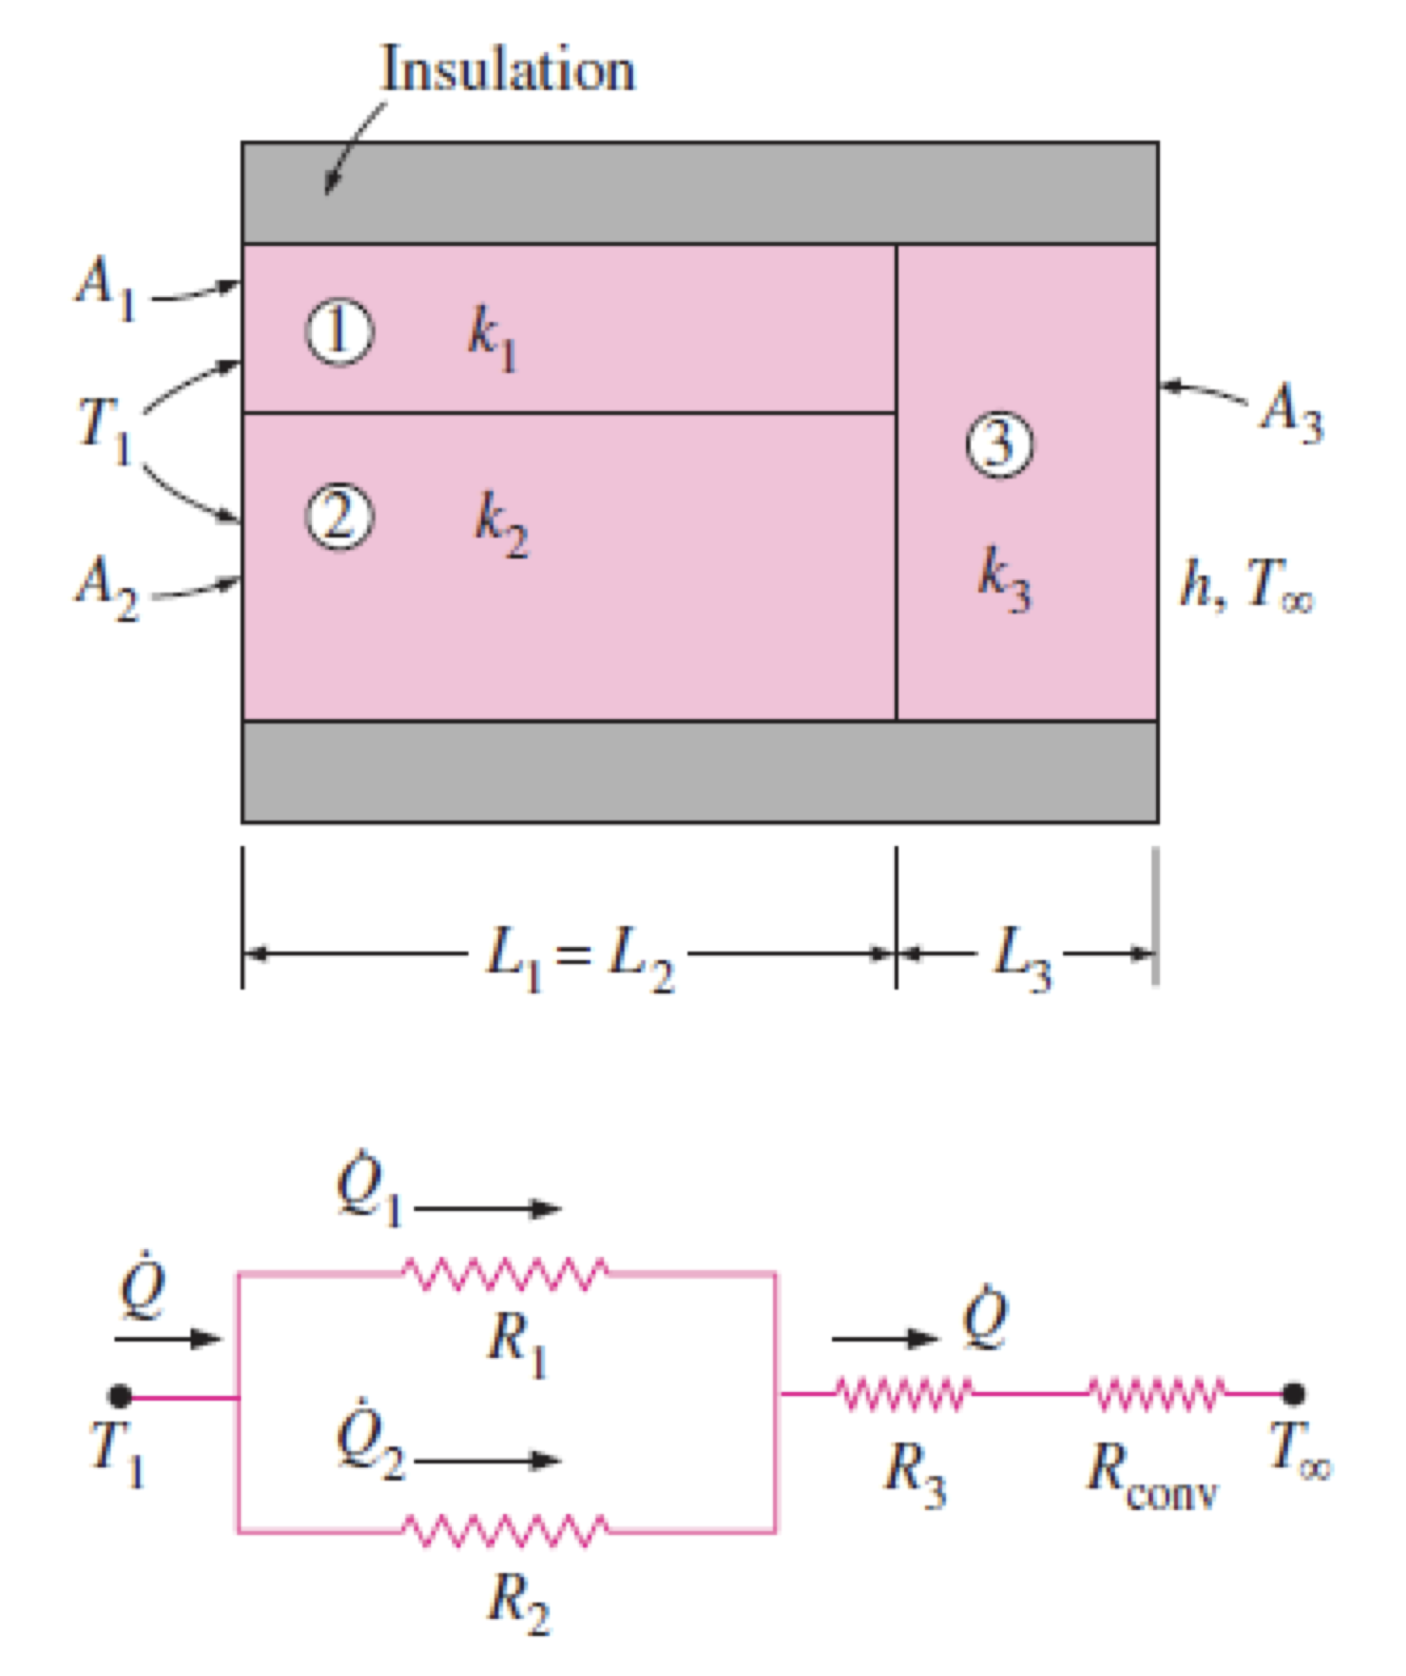
\includegraphics[width=0.7\linewidth]{images/thermal_resistance_parallel.png}
        \end{figure}
        \begin{align*}
            R_{tot} &= \frac{R_1 R_2}{R_1 + R_2} + R_3 + R_{conv} \\
        \end{align*}
        Note that in 1D analyses, we neglect the heat transferred between block 1 and 2.
    \end{itemize}
    \item For \color{red} cylinders: \color{black}
    \begin{figure}[H]
        \centering
        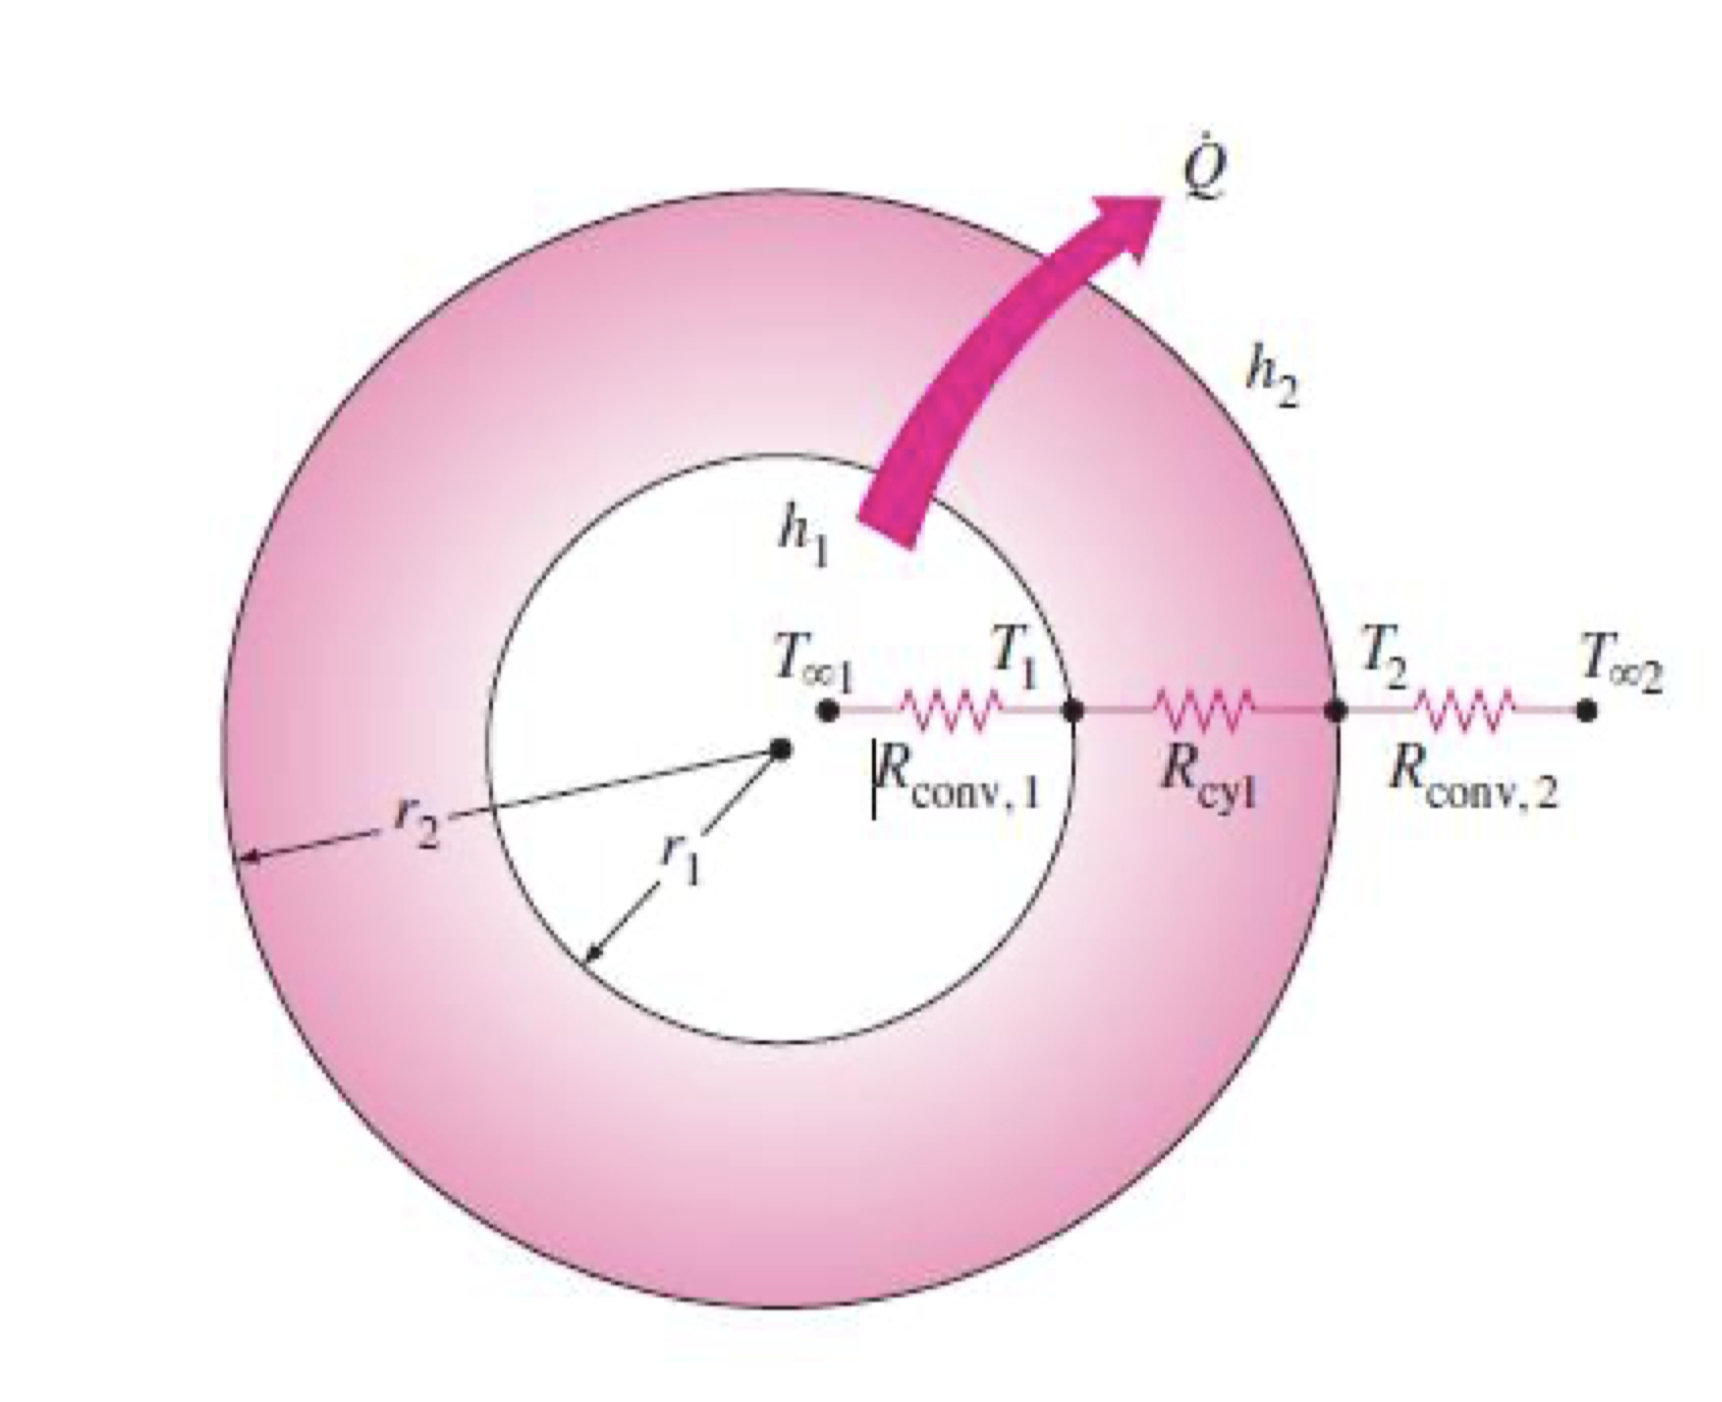
\includegraphics[width=0.9\linewidth]{images/thermal_resistance_cylinder.png}
    \end{figure}
    \begin{align*}
        R_{\text{cyl,cond}} &= \frac{\ln(r_2/r_1)}{2\pi L k} \\
        R_{tot} &= R_{conv,1}+R_{\text{cyl,cond}} + R_{conv,2} \\
        &= \frac{1}{(2\pi r_1 L)h_1} + \frac{\ln(r_2/r_1)}{2\pi L k} + \frac{1}{(2\pi r_2 L)h_2}
    \end{align*}
    \item For \color{red} sphere: \color{black}
    \begin{figure}[H]
        \centering
        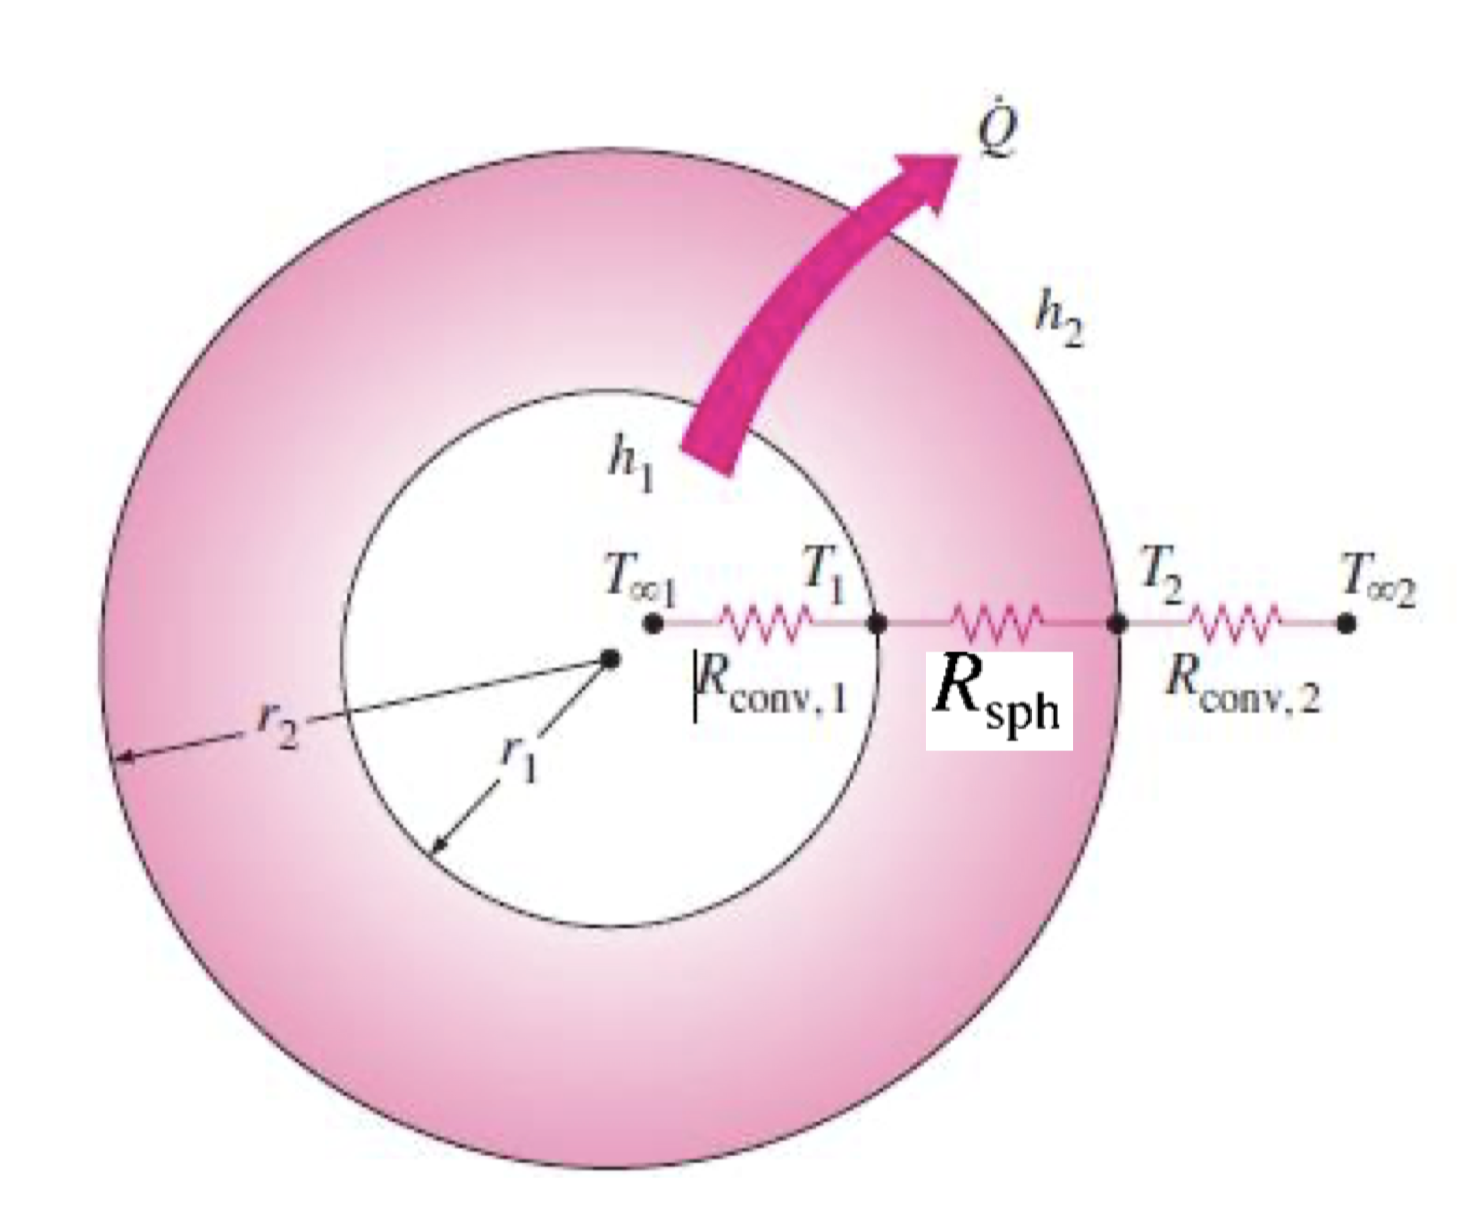
\includegraphics[width=0.9\linewidth]{images/thermal_resistance_sphere.png}
    \end{figure}
    \begin{align*}
        R_{sph} &= \frac{r_2 - r_1}{4\pi r_1 r_2 k} \\
        R_{tot} &= R_{conv,1} + R_{sph} + R_{conv,2} \\
        &= \frac{1}{(4\pi r_1^2)h_1} + \frac{r_2 - r_1}{4\pi r_1 r_2 k} + \frac{1}{(4\pi r_2^2)h_2}
    \end{align*}
    \item For \color{red} radiations: \color{black}
    \begin{align*}
        \dot{Q}_{rad} &= h_r A_s (T_s - T_{surr}) \\
        R_{rad} &= \frac{1}{h_r A}
    \end{align*}
\end{itemize}


